%sec1

\section{抄録を作成する際の注意事項}
論文抄録とは,簡易なことばで表現すると「論文を要約して書き出したもの」である.
同じように論文を要約した者としては,論文要旨が存在する.
宮治研では節や図表などの論文の体裁に近い形でのものを「抄録」と,節や図表などの情報が記載されていないものを「要旨」とよんで区別している.
社会情報学部では,宮治研でいうところの論文抄録を,論文要旨ということばで指示することがあるため,注意が必要である.

抄録は,論文と同じような見た目ではあるが,その要約の関係から論文の章や節の構成が異なる(ことが多い).
また,論文とは異なる書き方のルールが存在することに注意が必要である.
特に,抄録内の図表は,そのページの上または下に載せる.
ここで,図表が複数存在する場合には,上下に分散して配置されても良いし,それらが縦方向にまとめて並べられてもよい.

以上の点については,Word・\LaTeX のどちらで抄録を作成するにせよ,守る必要がある.

卒業研究の抄録(要旨)の Wordの雛形ファイルおよび \LaTeX のスタイルパッケージは Dropbox上に配置した.
同じフォルダ上に置いた仕上がりのPDFイメージを確認してから作業をすること.また,\LaTeX にて文書を作成する者は,本文書の残りの部分の利用方法および注意事項に目をとおすこと.

%sec2

\section{宮治研 抄録\LaTeX スタイルパッケージの使い方}
基本的に論文のスタイルパッケージと同様に作業をすれば良い.
例えば,\verb+main.tex+ファイルに必要事項を記載し,適切なファイルを取り込むように指定し,バッチコマンドを利用すれば,PDFファイルが出来上がる.

なお,抄録を記述する際注意事項として,スタイルパッケージの利用方法以外については次節にて解説する.

\subsection{サブタイトル有りの場合}
配布したファイルは,サブタイトルがある場合のサンプルになっている.
各自の 年度,学籍番号,氏名,タイトル,サブタイトルを所定の命令内に記入する.
\begin{screen}
{\small
%footnotesize
\begin{verbatim}
\nendo{2013年度}
\snum{15387019}
\jname{宮治 裕}
\thesistitle{宮治研における論文作成について}
\thesissubtitle{\LaTeX の利用}
\SUBTtrue
%\SUBTfalse
\end{verbatim}
}
\end{screen}

\subsection{サブタイトル無しの場合}
サブタイトル有りの場合と比較して3箇所の変更が必要である.
\begin{enumerate}
\item サブタイトルを記入する命令の先頭部分に \verb+%+ 記号を入れ,コメントアウト状態にする
\item \verb+\SUBTtrue+の前に\verb+%+ 記号を入れ,コメントアウト状態にする
\item コメントアウト状態の \verb+\SUBTfalse+の直前の \verb+%+ 記号を削除する
\end{enumerate}
以上の変更を行った設定を,以下に示す.
\begin{screen}
{\small
%footnotesize
\begin{verbatim}
%\thesissubtitle{}
%\SUBTtrue
\SUBTfalse
\end{verbatim}
}
\end{screen}

%sec3

\section{\LaTeX で抄録を作成する上での注意事項}
\LaTeX ので抄録を作成するうえでの注意事項について,主要なポイントについて記す.

\subsection{一番大きな文章単位: 節}
論文と抄録では,文章を作成する際のスタイルファイルが異なる.
宮治研の\LaTeX スタイルパッケージにおいて,論文では\verb+jsbook.cls+を,抄録においては\verb+jsarticle.cls+を用いている.

ここで,\verb+jsarticle.cls+を利用する際には,「章(\verb+\chapter{}+)」を利用することができない.
したがって,一番大きな枠組みとして「節(\verb+\section{}+)」を利用することになる.

\subsection{図表の位置の指定}
論文を書く際には,図や表の位置は本文中の記載よりも後であれば,特に気にする必要はなかった.
そのため,\verb+\begin{figure}[htbp]+の様に記述し,h(この場所)t(ページ上部)b(ページ下部)p(1ページ)の順の優先順位で図の位置を指定していた.

しかし,抄録の場合,図や表の位置は論文の上部や下部にまとめるようにする.
その為,\verb+\begin{figure}[b]+もしくは\verb+\begin{figure}[t]+のように指示をする必要がある.

なお,図の文字サイズは,本サンプルファイル程度の小ささが限界と考えること.

\begin{screen}
{\small
\begin{verbatim}
\begin{figure}[b]
\centering
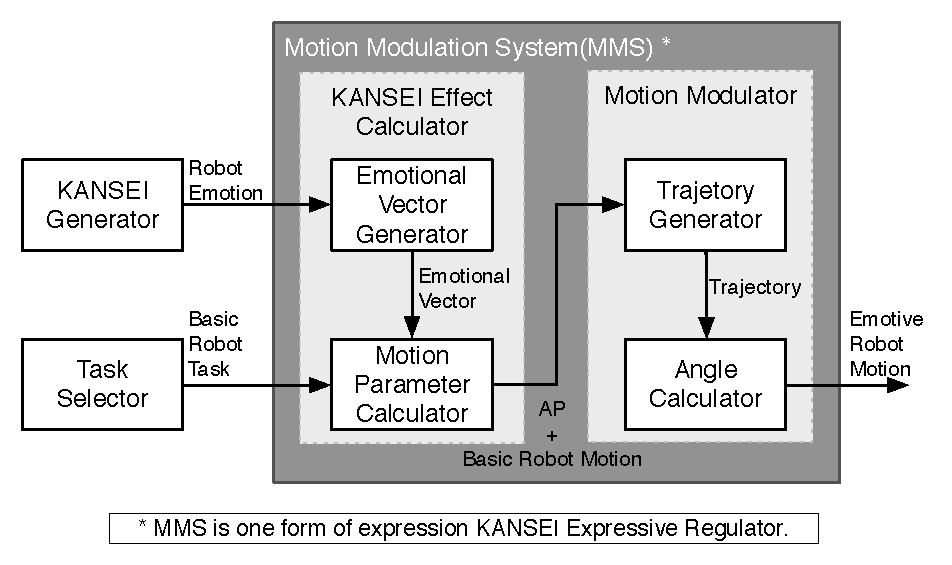
\includegraphics[width=8cm]{MMS.eps}
\vspace{-8mm}
\caption{MMSの内部構成}
\label{fig:mms}
\vspace{2mm}
\end{figure}
\end{verbatim}
}
\end{screen}

\begin{figure}[b]
\centering
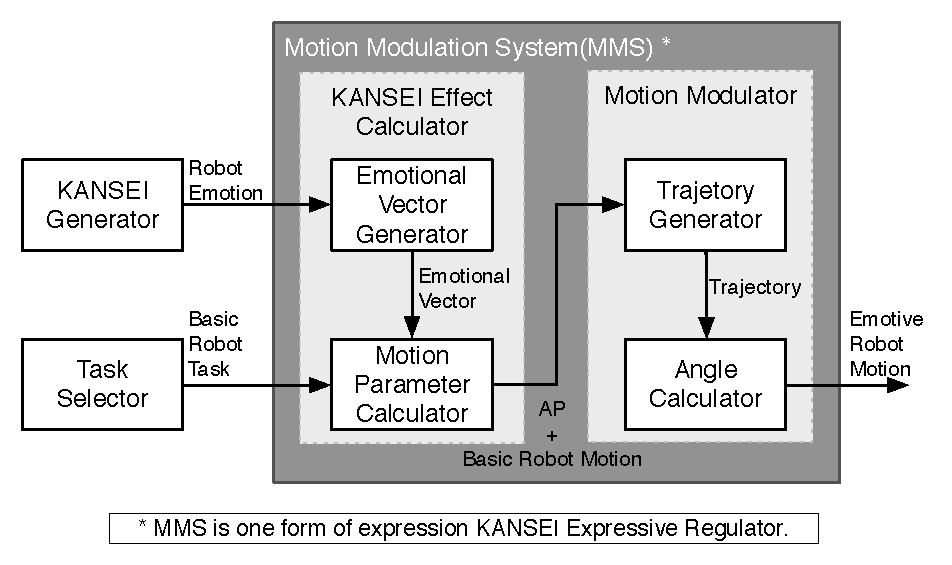
\includegraphics[width=8cm]{MMS.eps}
\vspace{-3mm}
\caption{MMSの内部構成}
\label{fig:mms}
\vspace{5mm}
\end{figure}

%sec4

\section{その他}
その他の事項として,本節では表の記述方法と参考文献について記載する.

\subsection{表の記述}
論文を記述する際にも指摘したが,表においては数値は右詰にしなければならない.また,ラベル部は中央揃えとすることが多い.

そのような設定をしたものを 表~\ref{table:face_rec}に示す.

\begin{table}[b]
\centering
\caption{WHLACによる顔表情認識率}
\label{table:face_rec}
\vspace{2mm}
\small
\begin{tabular}{|r|r|r|r|} \hline
\multicolumn{1}{|c|}{Data \#} & \multicolumn{1}{c|}{Ave.} & \multicolumn{1}{c|}{Max.} & \multicolumn{1}{c|}{Min.} \\ \hline\hline
1 &  0.67 (N/A) & 0.91 (39) & 0.46(21) \\ \hline
2 & 0.37 (N/A) & 0.50 (38) & 0.09(10) \\ \hline
3 & 0.65 (N/A) & 0.87 (45) & 0.28(10) \\ \hline\hline
\multicolumn{1}{|c|}{Total Ave.} & 0.56 & 0.76 & 0.27 \\ \hline
\end{tabular}
\end{table} %

\subsection{参考文献について}
抄録においては,参考文献のフォーマットも省略することが多いのだが,今回は論文時と同様の表記にて提出することとした.

参考文献を記載するファイルは新たに作成せず,論文と同じ \verb+myrefs.bib+ファイルをスタイルパッケージのフォルダにコピーし,しかるべき引用命令を入れれば良い.
サンプルとして,論文\cite{Kogami2009},書籍(の一部)\cite{WelfareJapan},書籍\cite{Nakata2010},予稿集\cite{Miyaji2003ROMAN},その他(Webサイトなど)\cite{HTUlatex}を組み込んだ.
